\documentclass[a4paper,14pt,fleqn]{article}%fleqn pour aligner les equations à gauche
\usepackage{../../Styles/Eval}


\newcommand{\chnum}{Chapitre 5 et 18}
\newcommand{\chtitle}{Transformations nucléaires et Diffractions/interférences}
\newcommand{\dtype}{DS 4}

\begin{document}
\maketitle
\section{Diffraction par une poudre de cacao}
On attribue la découverte de la diffraction à Francesco Grimaldi (1618-1663). Le but de l'exercice est d'étudier une application pratique de la diffraction : la détermination de la taille moyenne de poudre de cacao par granulométrie.\\
Les deux parties de l'exercice sont indépendantes.

\begin{figure}[h!]
    \caption{Granulomètre laser}
    \begin{minipage}{.4\linewidth}
    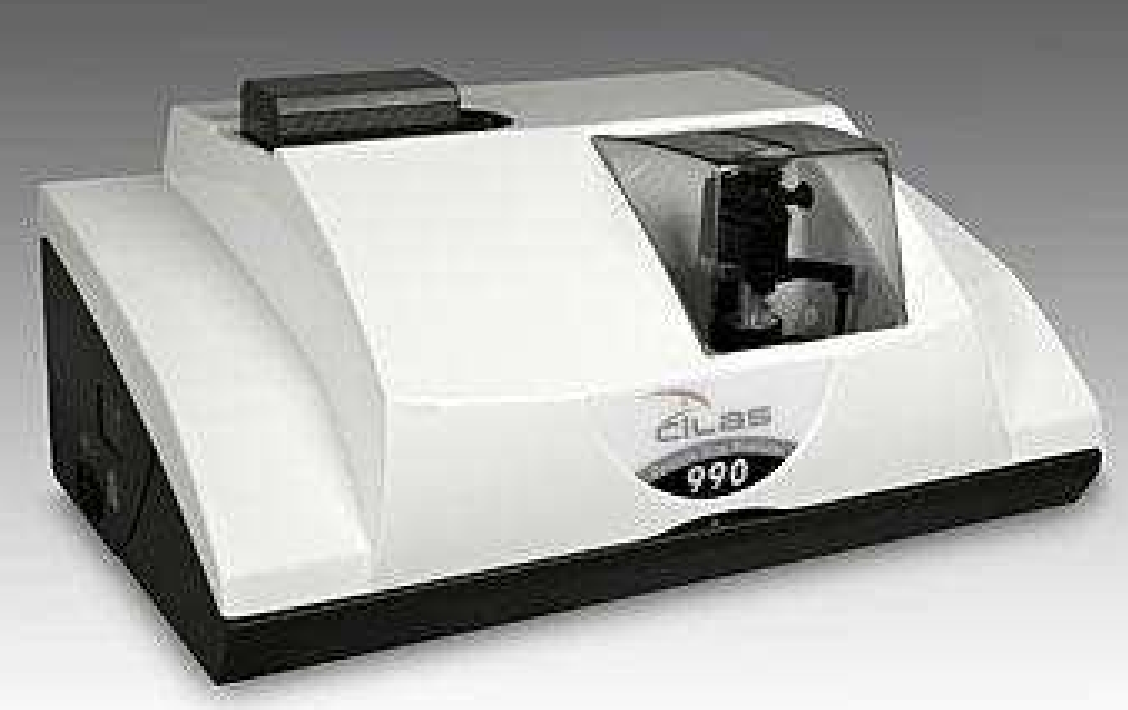
\includegraphics[width=\linewidth]{Ressources/TSPE_DS2b_Fig4.PNG}
    \end{minipage}\hspace{.02\linewidth}
    \begin{minipage}{.48\linewidth}
    L'appareil ci-contre permet de mesurer la taille de particules allant de \SI{40}{nm} à \SI{2500}{\micro\meter} tout en occupant un encombrement extrèmement réduit.\\
    Le fabricant de l'appareil indique que deux diodes laser de longueur d'onde \SI{635}{nm} et \SI{830}{nm} sont utilisées dans cet instrument de mesure.
    \end{minipage}
\end{figure}

\begin{figure}[h!]
    \caption{Différents types de chocolat}
    Le succès du chocolat, auprès des consommateurs, est lié à des caractéristiques gustatives bien identifiées mais aussi à la granulométrie de chacun des constituants.\\
    Cette dernière propriété représente un enjeu important du procédé de fabrication puisque des particules trop finement broyées rendront le chocolat collant alors que de trop grosses particules lui donneront un aspect granuleux à l'\oe il et en bouche.\\
    La mesure de la taille des particules, par diffraction laser, est une technique simple et rapide, adaptée à la détermination de la distribution granulométrique de tous les types de chocolat comme les chocolats de couverture utilisés pour le nappage, les chocolats au lait ou les chocolats utilisés pour les recettes instantanées.\\
    \begin{center}
        \begin{tabular}{|c|c|c|c|}
            \hline
            Type de chocolat & De couverture & Au lait & Aggloméré\\
            \hline
            $a$ (*) en \unit{\micro\meter} & 10 & 30 & 300\\
            \hline
        \end{tabular}
    \end{center}
    (*) $a$ représente le diamètre moyen recommandé de la poudre de cacao pour un type de chocolat.
\end{figure}

\begin{figure}[h!]
    \caption{Le z-score}
    Le z-score permet de comparer une valeur expérimentale à une valeur théorique en tenant compte des incertitudes associées. Il est défini par la relation suivante : $$ z = \dfrac{|x_{\text{expérimentale}} - x_{\text{théorique}}|}{u(x)} $$
    Si $z > 2$, on considère que la valeur expérimentale est en accord avec la valeur théorique.
\end{figure}

    \subsection*{Partie 1 : Vérification de la longueur d'onde d'une des diodes laser utilisées}
    L'objectif de cette partie est de vérifier la valeur de la longueur d'onde $\lambda$ d'une des diodes laser utilisées dans l'appareil de granulométrie. Sur le trajet du faisceau laser, on intercale des fils de différents diamètres. Sur un écran placé à une distance $D$, on observe une figure de diffraction.\\
    $L$ représente la largeur de la tache centrale et $\theta_0$ le demi-angle au sommet exprimé en radian.

    \begin{enumerate}
        \item \begin{enumerate}
            \item Rappeler les principales propriétés du faisceau d'un laser.
            \item Pour une longueur d'onde donnée, déduire l'évolution du demi-angle $\theta_0$ en fonction du diamètre $a$ du fil. Donner la relation qui lie $\lambda$, $\theta_0$ et $a$.
            \item On fait l'hypothèse que l'angle $\theta_0$ est petit. Dans ce cas, on peut écrire $\tan \theta_0 \approx \theta_0$ avec $\theta_0$ en radian.\\
            A l'aide du schema, démontrer que la largeur de la tache centrale est donnée par l'expression : $$ L = k \cdot \dfrac{1}{a} $$
            avec $k =  2 \lambda \cdot D $
            \item Expérimentalement, on mesure la largeur de la tache centrale $L$ pour des fils calibrés de différentes valeurs de diamètre $a$. On porte les valeurs obtenues dans le graphique ci-dessous. A partir du graphique, déterminer la longueur d'onde $\lambda$ de la diode laser utilisée.
            \item L'incertitude absolue sur la longueur d'onde $\lambda$, notée $u(\lambda)$, peut être déterminée à partir de la relation suivante : $$ u(\lambda) = \lambda \cdot \sqrt{\left(\dfrac{u(D)}{D}\right)^2 + \left(\dfrac{u(k)}{k}\right)^2}$$
            L'incertitude absolue sur la valeur du coefficient directeur est $u(k) = \SI{1,2E-7}{\meter\squared}$.\\
            Exprimer la valeur de la longueur d'onde $\lambda$ avec son incertitude. Confronter aux valeurs donnnées par le fabriquant de l'appareil en calculant le z-score puis conclure.
        \end{enumerate}
    \end{enumerate}

    \begin{figure}[h!]
        \caption{Représentation de l'évolution de la largeur de la tache centrale de diffraction en fonction de l'inverse de l'épaisseur des fils calibrés.}
        \begin{center}
            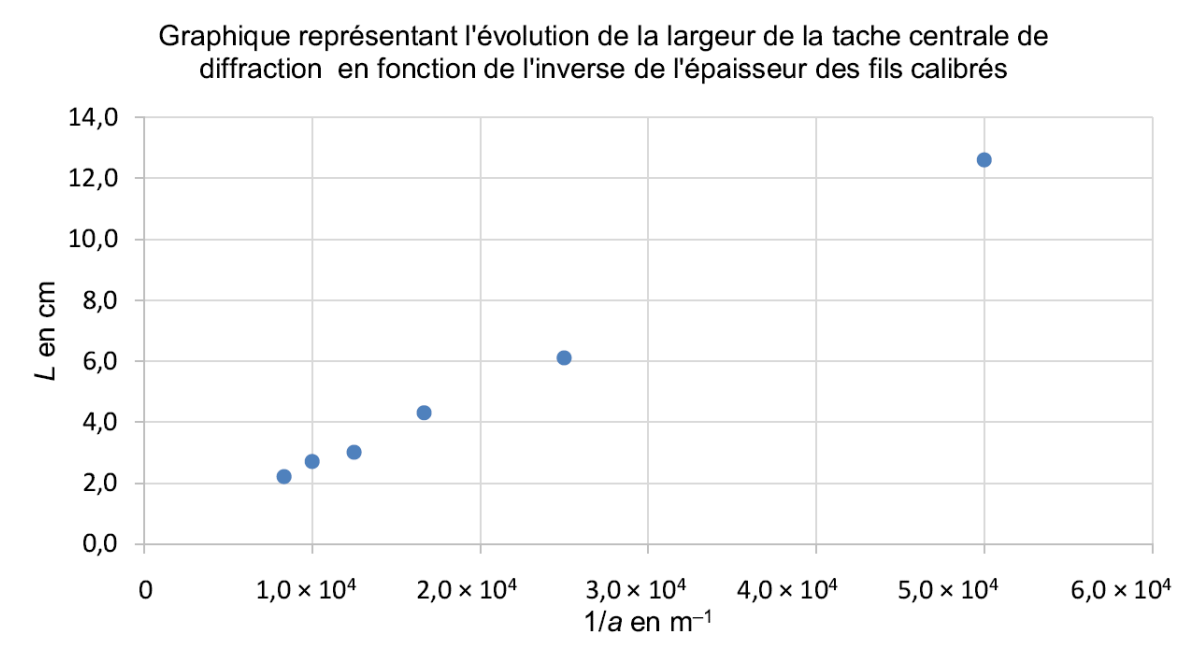
\includegraphics[width= .8\linewidth, trim = 0 0 0 2.5cm,clip]{Ressources/TSPE_DS2b_Fig6.PNG}
        \end{center}
    \end{figure}

    \subsection*{Partie 2 : Etude de la diffraction apr la poudre de cacao}
    Dans cette partie, on considère que l'on peut déterminer le diamètre moyen des grains de cacao d'une poudre donnée en utilisant une figure de diffraction réalisée avec la diode laser de longueur d'onde $\lambda = \SI{635}{nm}$.

    \begin{figure}[h!]
        \caption{Expérience de diffraction par un trou circulaire}
        \begin{center}
            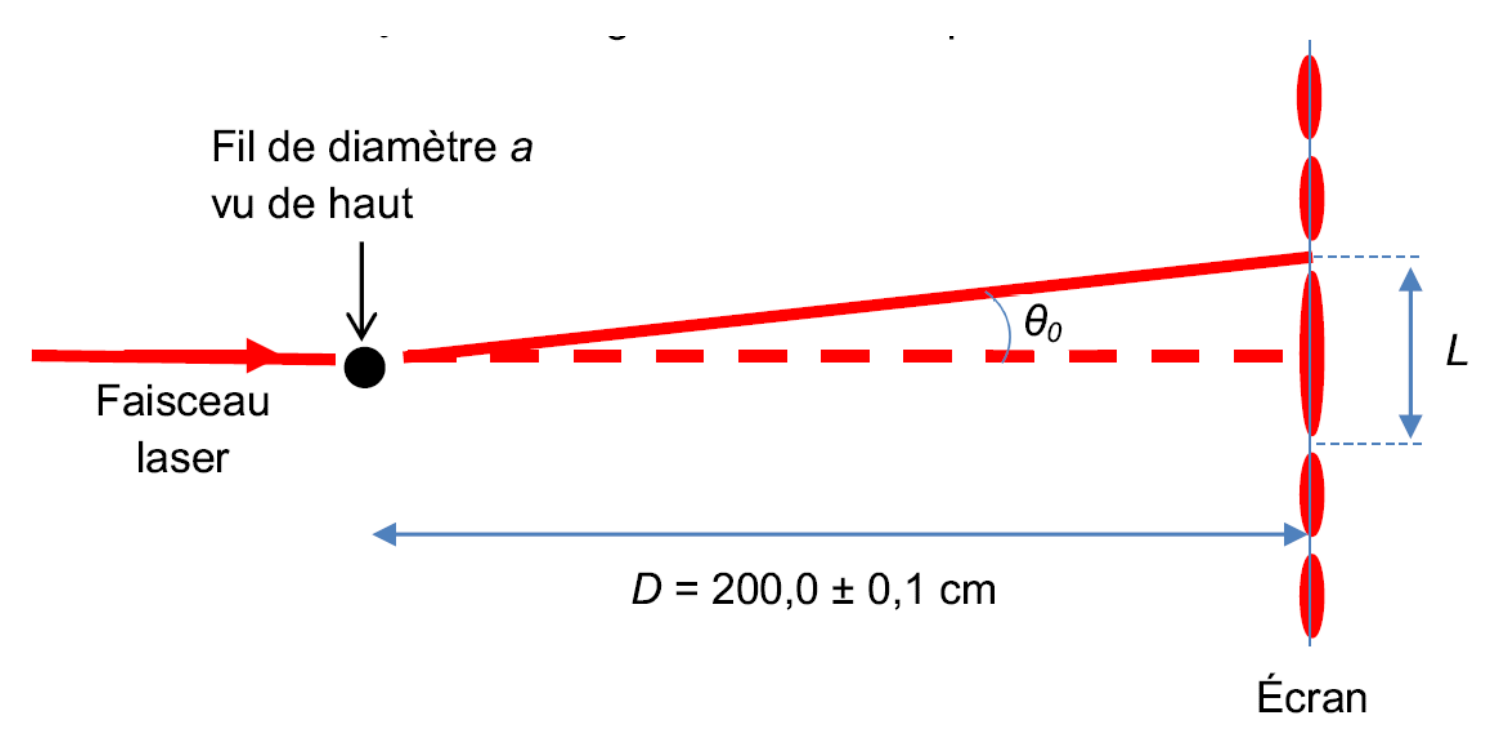
\includegraphics[width = .6\linewidth]{Ressources/TSPE_DS2b_Fig5.PNG}
        \end{center}
        La figure de diffraction obtenue par un trou circulaire est constituée de cercles concentriques alternativement brillants et sombres avec : $$ \sin \theta_0 = \dfrac{1,22 \cdot \lambda}{a} $$
        $\lambda$ : longueur d'onde du faisceau laser, exprimée en mètre\\
        $a$ : diamètre du trou, exprimé en mètre\\
        $\theta_0$ : demi-angle au sommet, exprimé en radian
    \end{figure}

    \begin{enumerate}[resume]
        \item \begin{enumerate}
            \item En utilisant un montage proche de celui donné ci-dessous, on réalise l'expérience sur un échantillon de poudre de cacao. Sachant que les grains de cacao sont assimilés à des sphères, justifier le fait qu'on observe une figure de diffraction identique à celle obtenue avec un trou circilaire.
            \item Après traitement informatique, des résultats expérimentaux lors du contrôle d'un échantillon de poudre de cacao, on obtient le graphe ci-après donnant l'intensité lumineuse relative sur l'écran en fonction du demi-angle $\theta_0$. Peut-on utiliser cet échantillon pour un chocolat de couverture ?
        \end{enumerate}
    \end{enumerate}

\begin{figure}[h!]
        \caption{Intensité lumineuse relative en fonction du demi-angle au sommet}
        \begin{center}
            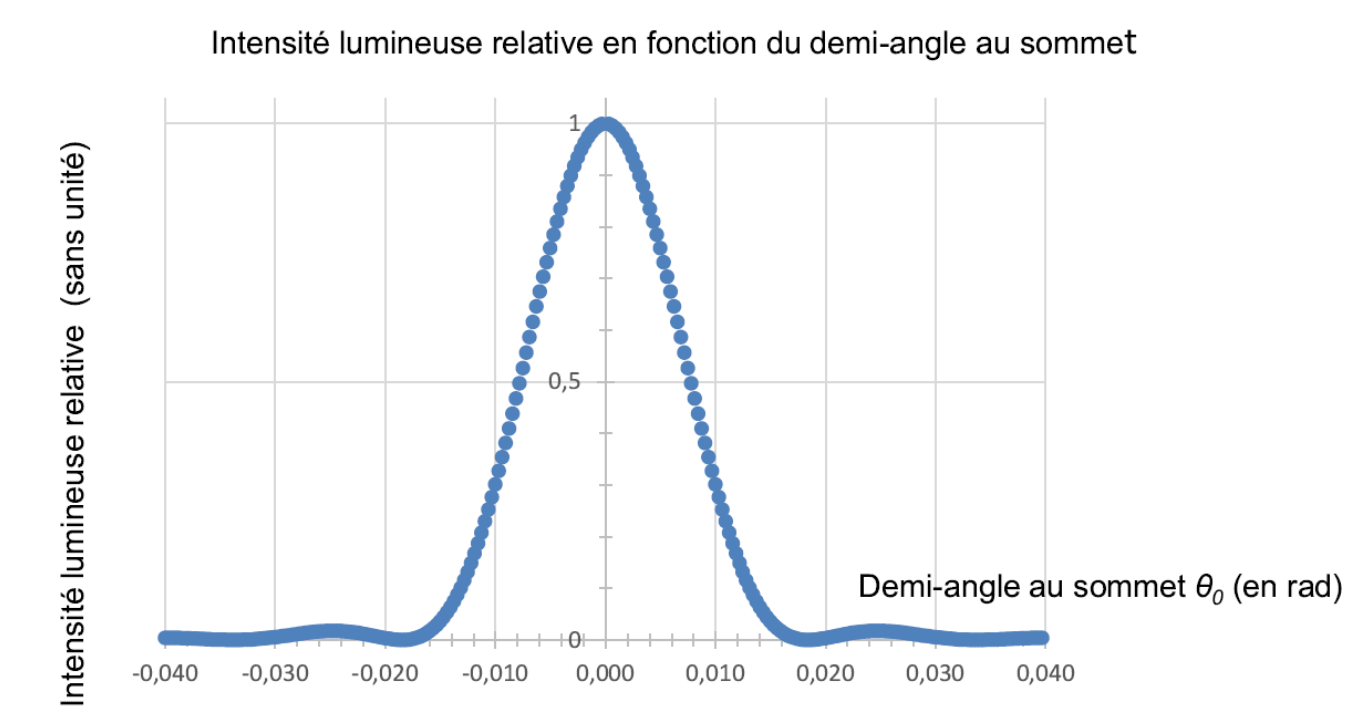
\includegraphics[width=.8\linewidth, trim = 0 0 0 2cm, clip]{Ressources/TSPE_DS2b_Fig8.PNG}
        \end{center}
        
\end{figure}

\pagebreak
\newpage
\section{Une potion radioactive}
De tous temps, certaines substances sont considérées comme des remèdes contre tous les maux, des panacées.\\
\begin{minipage}{.7\textwidth}
    Au début du 20\textsuperscript{e} siècle, le Radithor, sorte de "potion magique" était censé soigner plus d'une centaine de maladies.\\
    Un cancérologue américain a trouvé chez un antiquaire, plusieurs bouteilles de Radithor. Bien que vidées depuis 10 ans de leur contenu, les bouteilles se sont avérées être encore dangereusement radioactives. Chacune avait vraisemblablement contenu environ un microcurie de radium 226 et de radium 228\\
    1 microcurie correspond à \SI{3,7E4}{Bq}.
\end{minipage}
\begin{minipage}{.3\textwidth}
    \centering
        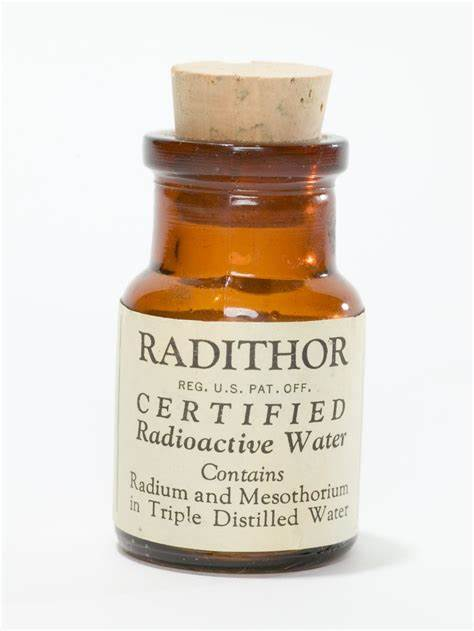
\includegraphics[width=.5\linewidth]{Ressources/TSPE_DS5_Fig1.jpg}
\end{minipage}

\begin{tabular}{|>{\centering}m{3cm}|c|c|c|c|c|}
     \hline \textbf{Noyau}&Radium 226&Radium 228&Actinium 228&Radon 222&Hélium 4\\
    \hline \textbf{Symbole}&\ce{^226_88Ra}&\ce{^228_88Ra}&\ce{^228_89Ac}&\ce{^222_86Rn}&\ce{^4_2He}\\
    \hline
\end{tabular}\\

\begin{tabular}{|>{\centering}m{3cm}|c|c|c|}
     \hline \textbf{Noyau}&Radium 226&Radon 222&Hélium 4\\
    \hline \textbf{Masse en $u$}&\num{225,9970}&\num{221,9703}&\num{4,0015}\\
    \hline
\end{tabular}
\begin{itemize*}
    \item \textbf{Unité de masse atomique} : $\SI{1}{u}=\SI{1,66054E-27}{kg}$
    \item \textbf{Célérité de la lumière dans le vide} : $c=\SI{3,00E8}{\meter\per\second}$
    \item \textbf{Constante d'Avogadro} : $N_A=\SI{6,02E23}{\per\mole}$
    \item \textbf{Masse molaire du \ce{^226_88Ra}} : $M=\SI{226}{\gram\per\mole}$
\end{itemize*}


\subsection{Le radium 226 et le médothorium}
Sur l'étiquette du flacon de Radithor est mentionnée la présence de mésothorium, ancienne dénomination du radium 228. Cette "eau certifiée radioactive" contenait également du radium 226.
\begin{enumerate}
    \item Les noyaux de radium 228 et de radium 226 sont des isotopes. Expliquer.
    \item Le radium 228 se désintègre pour donner l'isotope 228 de l'actinium \ce{Ac} et une particule notée \ce{X}. $$\ce{^228_88Ra -> ^228_89Ac + ^A_Z X}$$
Compléter l'équation de désintégration en justifiant puis identifier \ce{X}. De quel type de radioactivité s'agit-il ?
\end{enumerate}
Dans la suite de l’exercice, on néglige la présence de radium 228 dans le Radithor.\\ 
On suppose que l’activité radioactive du flacon est uniquement due à la présence de l’isotope 226 du radium. Celui-ci se désintègre spontanément selon l’équation suivante :
$$\ce{^226_88Ra -> ^222_86Ac + ^4_2He}$$

\subsection{Constante radioactive du radium 226}
 L’activité A(t) d’un échantillon de noyaux de radium 226 suit la loi de décroissance exponentielle $A(t)=A_0\cdot e^{-\lambda \cdot t}$, avec $A_0$ l'activité à $t=\SI{0}{s}$.
 \begin{enumerate}[resume]
     \item Rappeler la définition de la demi-vie $t_{1/2}$ d'un échantillon radioactif.
     \item Vérifier sur la courbe donnant l'évolution de l'activité de l'échantillon en fonction du temps représentée dans le \textbf{Figure~\ref{doc1}}, que la demi-vie du radium 226 est égale à \SI{1,60E3}{ans}.
     \item Établir la relation entre la demi-vie et la constante radioactive $\lambda$ puis calculer la valeur de $\lambda$ en \unit{\per\second}.
 \end{enumerate}
 \subsection{Masse de radium 226}
 \begin{enumerate}[resume]
     \item Donner la relation liant l'activité $A(t)$ d'un échantillon radioactif au nombre $N(t)$ de noyaux radioactifs présents.
     \item Calculer $N_0$, le nombre de noyaux de radium 226 initialement présents dans le flacon de Radithor.
     \item Vérifier que le flacon contenait alors une masse $m_0 = \SI{1,0}{\micro\gram}$ de radium 226.
 \end{enumerate}

 \begin{figure}[h!]
    \caption{Activité d’un échantillon de radium 226 en fonction du temps }
    \centering
    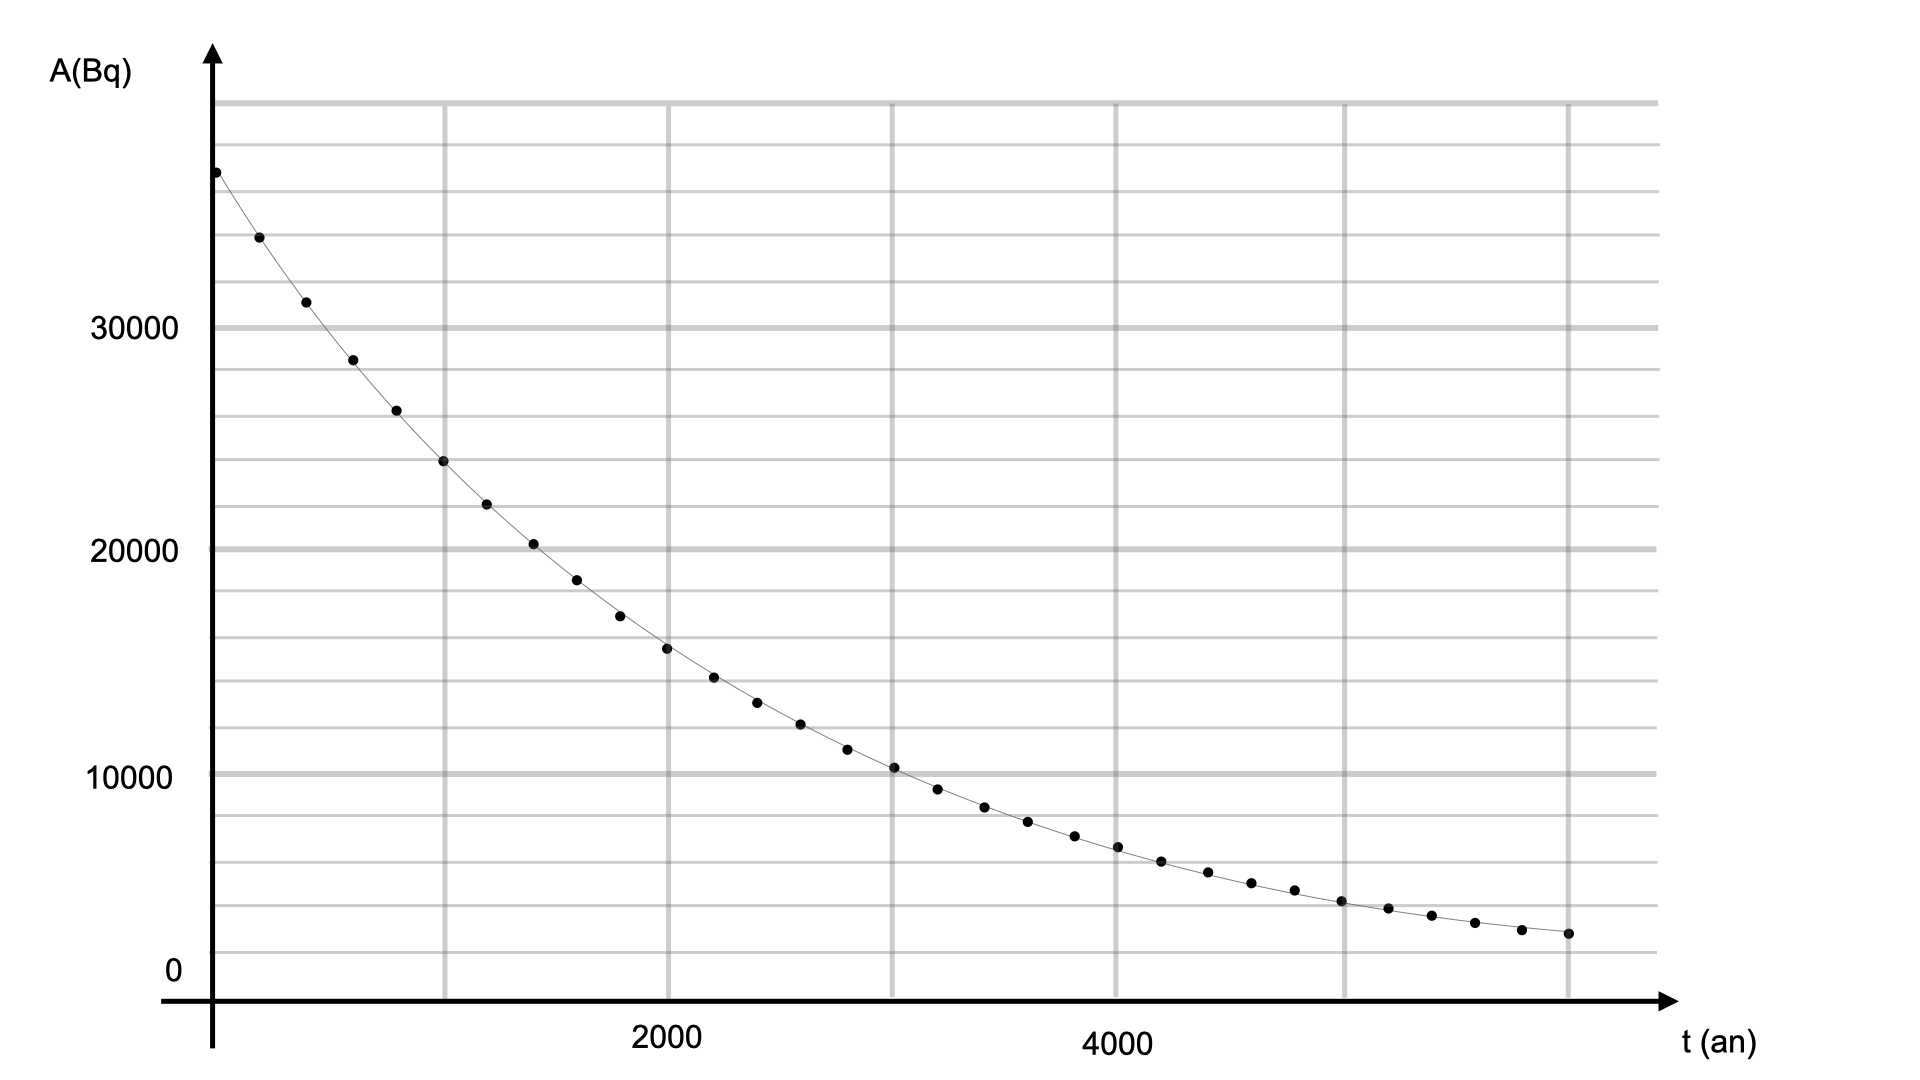
\includegraphics[width=.9\linewidth]{Ressources/TSPE_DS5b_Fig1.png}
    \label{doc1}
 \end{figure}

\end{document}